\chapter{Introduction}\label{ch:intro}


Human health and environmental quality are deeply linked. According to
the World Health Organization (WHO), in 2022 alone, at least 1.7 billion people
relied on contaminated drinking water sources, leading to an estimated 1 million
deaths from diarrhea. Additionally, ambient air pollution has emerged as the
leading environmental health risk, contributing to over 8 million deaths
annually \cite{air-pollution-mortality}. Addressing these challenges requires
data-driven decision-making. Yet, comprehensively modeling the complex physical
processes that drive changes in water and air quality at scales relevant to
human interactions is often computationally infeasible.

Despite this challenge, the environmental data volumes continues to expand
rapidly. For example, remote sensing platforms like Sentinel-2 generate
terabytes of multi-spectral imagery each day \cite{sentinel-2-data}. Next
generation systems, such as NASA’s recently launched PACE mission,
employ hyperspectral imagers capable of sampling \textit{hundreds} of individual
wavelength bands. At the same time, advancements in air quality measurement
technologies have led to a proliferation of new, low-cost sensors. Dense
networks of these sensors are being deployed across many urban areas to provide
real-time assessment of air quality dynamics. This wealth of data presents a
significant opportunity to inform environmental policy, with machine learning
techniques serving as a the primary tool to bridge the gap between our current
physical models and environmental data.




\section{Water Quality}

Water quality consists of the physical, chemical, and biological characteristics
of water, which characterize overall ecosystem health and its suitability for
uses such as drinking and agriculture. Poor water quality can result from a
range of anthropogenic and natural factors. Industrial pollution, particularly
from chemical manufacturing, mining, and agriculture, introduces
contaminants such as heavy metals, pesticides, and effluents into water
bodies \cite{schwarzenbach-water-pollution}. Urban runoff
picks up additional oils, plastics, and sediments, carrying them into
water sources where they cause a variety of issues such as
eutrophication and oxygen depletion \cite{smith-eutrophication}.
In addition to human activities, natural factors like soil erosion, volcanic
eruptions, and the leaching of naturally occurring metals from geological
formations can degrade water quality \cite{water-quality-natural}. Climate
change also plays a role, where increased water temperatures and altered
precipitation patterns contribute to the growth of harmful algal blooms
\cite{climate-change-water-quality}.

In situ and laboratory methods remain fundamental for water quality assessment,
providing direct and precise measurements for a variety of parameters. In situ
techniques involve the deployment of sensors and
instruments directly into water bodies to measure parameters such as pH,
dissolved oxygen, conductivity, and temperature. These sensors,
typically placed in monitoring stations or attached to buoys, often provide continuous
data streams essential for tracking short-term changes and local variability
\cite{in-situ-water-quality}. Portable instruments, such as multiparameter probes, are
also commonly used for spot measurements during field surveys, offering
flexibility in data collection across diverse environments. On the other hand,
laboratory analysis involves the collection of water samples which are then
transported to the lab for detailed examination.
Techniques such as mass spectrometry and liquid chromatography are used to
analyze heavy metals, pesticides, and organic compounds at
trace levels \cite{mass-spec-water, lc-ms}. Microbiological testing for harmful
pathogens is also used for assessing water safety, particularly for drinking
water \cite{microbio-methods}.

The key shortcoming of in situ and laboratory methods for 

Remote sensing methods offer a crucial advantage for addressing the limited
spatial coverage of in situ and laboratory measurements
Satellite and airborne sensors provide large-scale
observations that can cover vast water bodies, overcoming the spatial
constraints of point-based in situ monitoring stations. For instance, platforms
like Sentinel-2 and Landsat capture multispectral and hyperspectral imagery,
allowing for the estimation of key water quality indicators such as turbidity,
chlorophyll a, and suspended sediments over entire lakes, rivers, and coastal
areas \cite{}.


- key idea: remote sensing takes too long to generate fine-grained datasets

- most studies use limited in-situ sensing

- limitations of full radiative transfer simulation

- Summary of current limitations

- Need: ability to rapidly map pollutant concentrations to track contaminant
evolution and localize sources
- Need: ability to identify pollutant signatures from complex datasets


\section{Air Quality}

- growing problems for air quality

- contributers to poor air quality

- dissertation focus: Particulate Matter

\begin{figure}[h!]
  \centering
  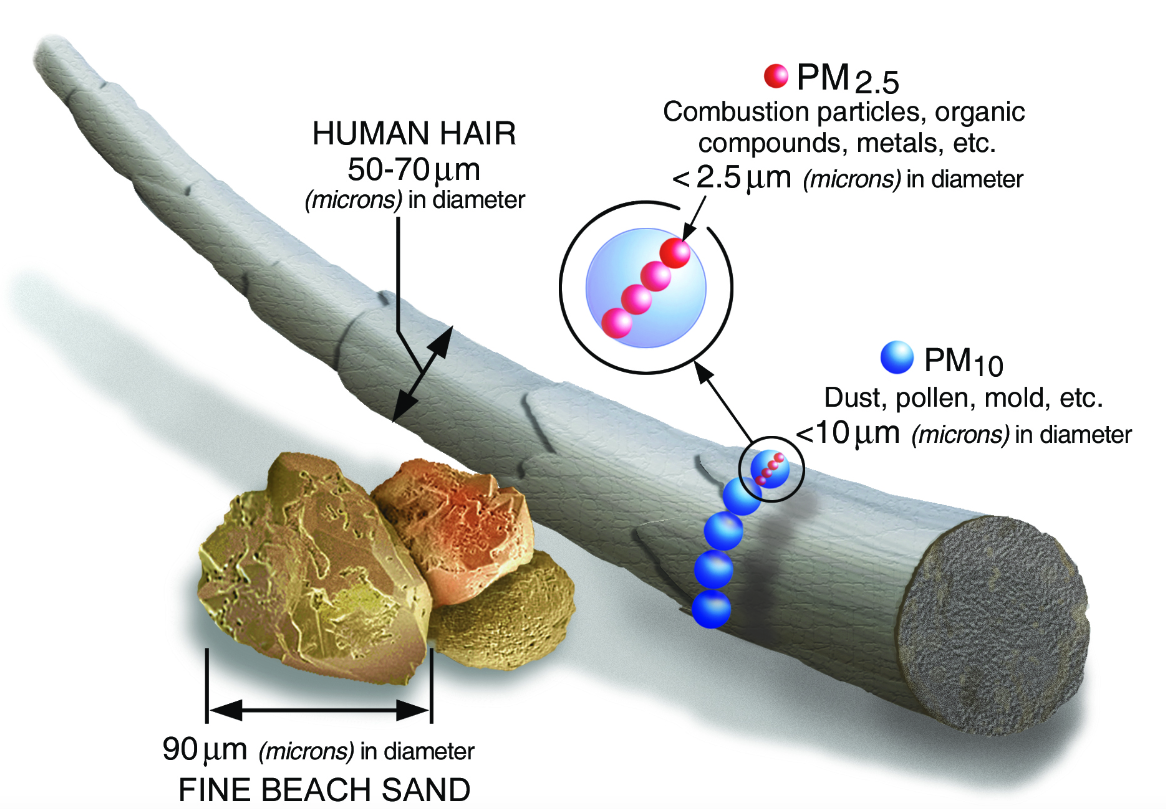
\includegraphics[width=0.75\columnwidth]{introduction/pm-size.png}
  \caption{Size comparisons for PM particles. Image source: US EPA
    (\url{https://www.epa.gov/pm-pollution/particulate-matter-pm-basics}, last
    accessed 2024-09-12).}
  \label{fig:pm-size-scale}
\end{figure}


- traditional approaches for PM monitoring

- FRM and FEM sensors (spatially and temporally limited)
- Satellite based PM estimation

% - Prabuddha et al. combine remote sensing observations for aerosol optical depth
% with meteorological data to predict ground level PM 2.5 using machine learning
% together with ground based-sensors \cite{prabuddha-pm-satellite}
% - Average US values exceeded 9 $\mu g/m^3$ standard 20\% of the time with the
% eastern US and California exceeding the limit over 50\% of the time during the
% sampling period from Jan. 2020 to June 2023.


- key idea: FRM and FEM sensors are too expensive to obtain measurements at
relevant spatial scales
- key idea: 24 hour averages are too infrequent to capture known temporal
patterns

- Need: low cost sensors which can be densely distributed in urban environments
to assess spatial variability.
- Need: computational tools to extract insights from PM data by understanding
\textit{local} trends.



% \begin{table}[h!]
%   \centering
%   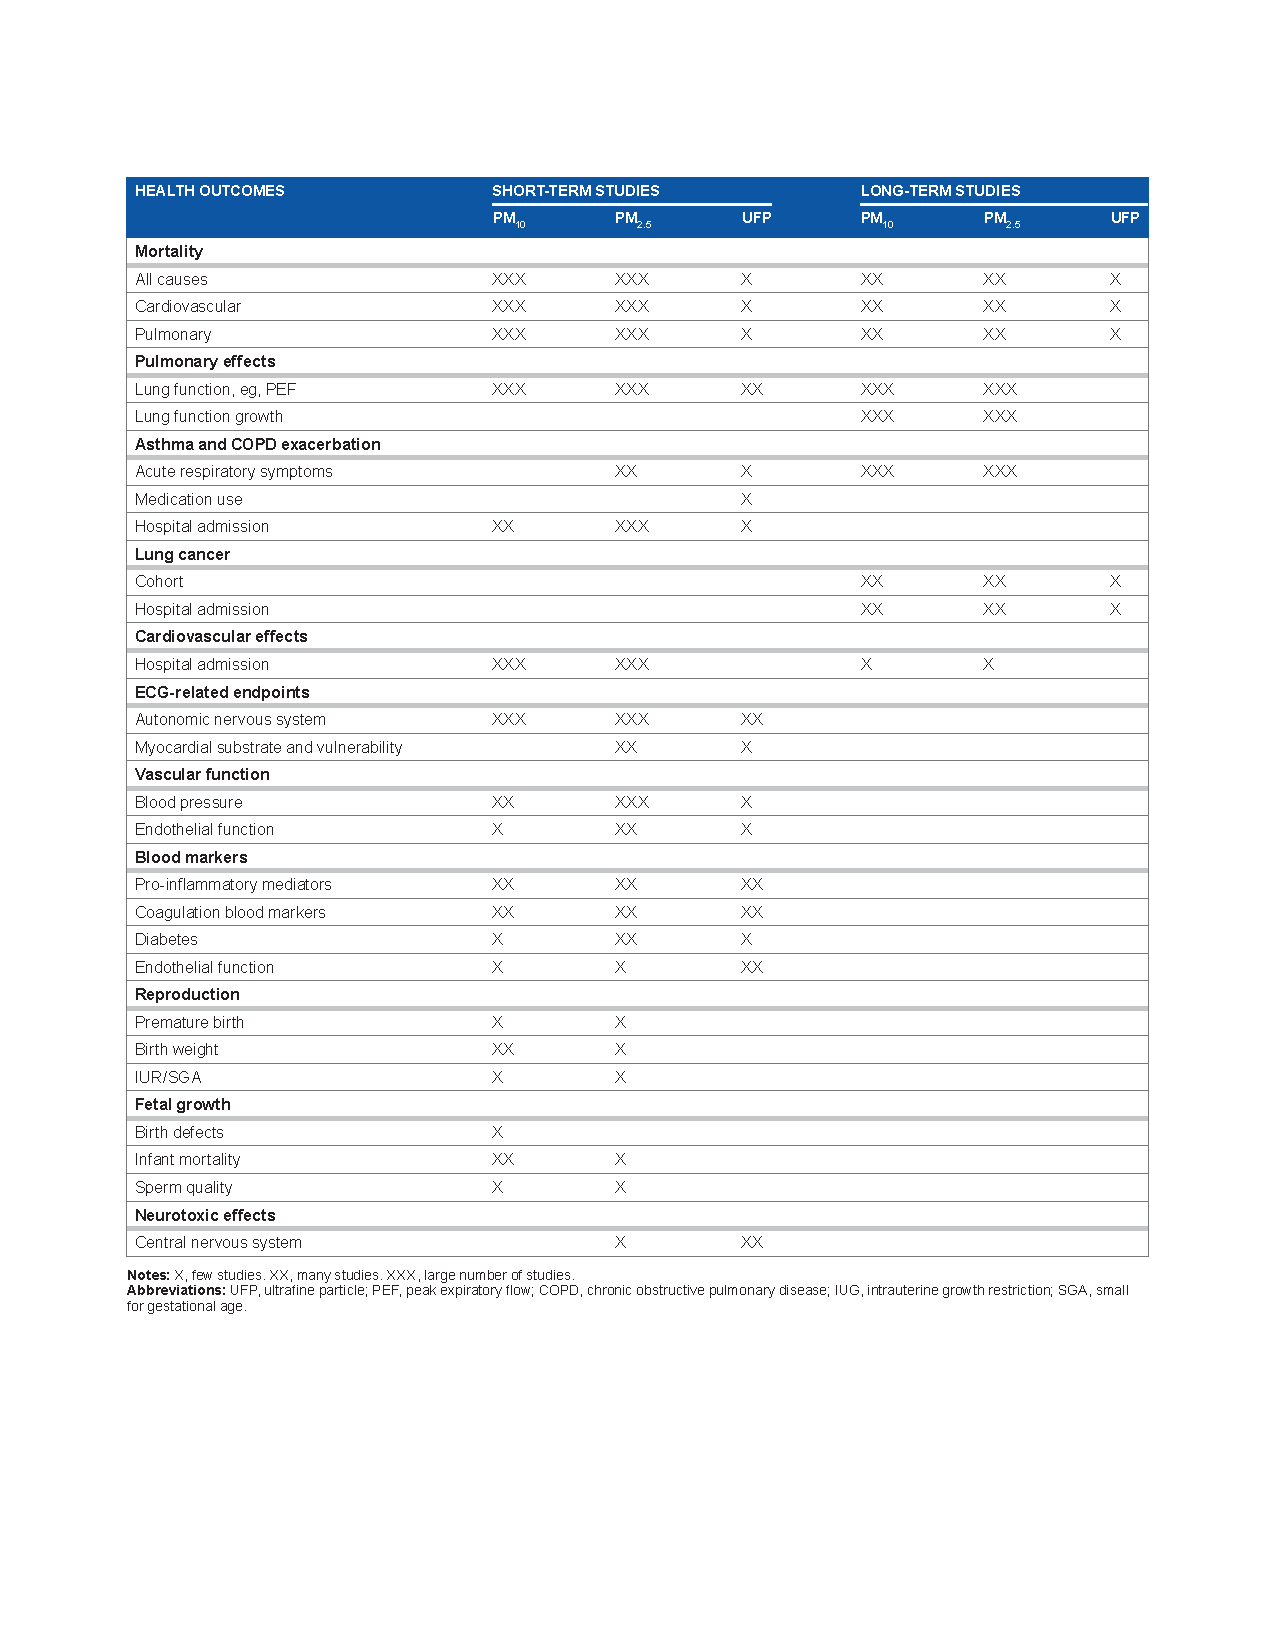
\includegraphics[width=\textwidth]{introduction/HealthEffectsParticulates.pdf}
% 	\caption{Tabular literature review of particulate matter and health outcomes related to PM$_{10}$, PM$_{2.5}$, and ultrafine particulates (UFPs) exposure (based on the literature review of \cite{Lary:2015}).}
% 	\label{Table.HealthEffectsParticulates}
% \end{table}


\section{Machine Learning}

- what is machine learning
- role of machine learning in physical sciences
- define physics-based machine learning (broadly defined)
   - we refer to physics-based machine learning as machine learning models
   developed specifically for data from physical sensors (e.g. not image
   classification or text generation).
   - Particularly important for physics-based machine learning applications is
   - model interpretability
   - uncertainty quantification

In recent years machine learning has exploded in popularity becoming entwined in
almost every aspect of our lives from image recognition on social media sites,
to the now ubiquitous large large language models like ChatGPT. Because the
field is so wide, many of the most popular machine learning models must be
generic enough so as to apply to \textit{any} well defined regression or
classification task. For example, the problem of image classification is
incredibly challenging if we do not impose any restrictions on the type of
content represented in our data, as illustrated in Figure
\ref{fig:dog-or-muffin}.

\begin{figure}[!hbt]
  \centering
  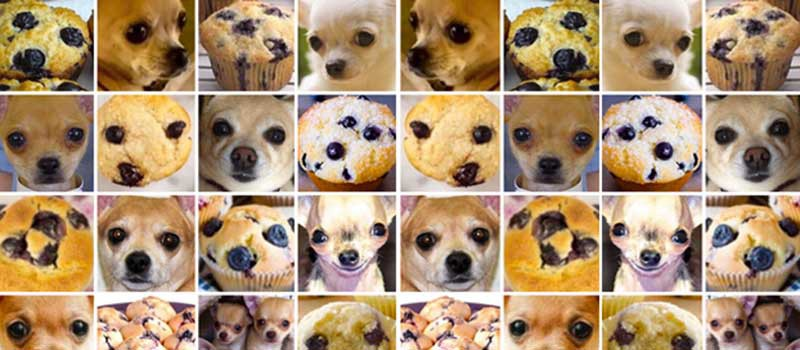
\includegraphics[width=0.6\columnwidth]{introduction/dog-or-muffin.jpeg}
  \caption{A classic machine learning meme comparing pictures of Chihuahuas with muffins illustrating the potential difficulties faced by generic image classification tasks.}
  \label{fig:dog-or-muffin}
\end{figure}
As a consequence, we typically can not expect a machine learning model to
generalize beyond the bounds of their training data.


In the realm of scientific applications, this is often \textit{not} the case;
the universe is well described by deep physical principles with underlying
mathematical symmetries and structures. Therefore, rather than throwing away all
of our prior scientific knowledge for each machine learning task, we can instead
develop techniques which enable us to directly or indirectly impose physical
requirements on our machine learning models. Similarly, we can utilize machine
learning to gain insight into physical processes where a first principles
relationship has not yet been established. Together these ideas are known as
\textit{Physics-Based Machine Learning} or more generally \textit{Scientific
  Machine Learning} (SciML for short) and provides us the exact set of tools
needed to marry scientific models together with data to produce actionable
insights \cite{rackauckas2020universal}.

- physics-based machine learning involves
  - physics informed / scientific machine learning
  - physically motivated model selection
  - robust uncertainty quantification either by using probabilistic models or by
  using methods to infer prediction uncertainties.


% Successful physical theories are predictive, explainable, and quantifiable (i.e.
% uncertainty can be characterized). Most machine learning tasks involve abstract
% data for which this can be challenging. A physics-based machine learning
% approach involves model selection, uncertainty quantification, physical
% reasonableness, etc..


% The general problem of ML is hard with when no structure is assumed on data (include example of pit bull or potato)

% For situations involving data from physical sensors describing real systesm, physics tells us there are underlying rules which govern the dynamics of real systems

% When applying ML we should therefore place a high value on physics-based models, i.e. machine learning models tailord for the specific physical system, rather than generic abstract algorithms. This is important in all stages of the ML pipeline from feature selection (Robot team supervised), dimensionality reduction (i.e. the latent space of the GTM and GSM), model selection, model evaluation, etc. In summary:

% \begin{itemize}
%   \item Prefer interpretable models (e.g. deicsion trees) to black boxes
%   \item Prefer probabilistic models (e.g. GTM vs SOM) to deterministic models (all data has uncertainty and no model is perfect)
%   \item Prefer models which incorporate prior knoweldge of the physical system such as dynamical laws, symmetries, natural constraints, etc. This is specifically known as \textbf{physics-informed} machine learning or \textbf{scientific machine learning}  (SciML).
% \end{itemize}



\section{Dissertation Goals}

The goal of this dissertation is to advance physical sensing in service of
society by developing physics-based machine learning methods for the analysis
of environmental data. Towards this end, this work presents a collection of case
studies utilizing both supervised and unsupervised machine learning techniques
to produce actionable insights in the context of water quality and air quality.

For the water quality domain, our primary goal is to develop methods to translate
spectroscopic measurements directly into the abundance of contaminants. 



Applications of this research center on addressing basic questions using
observational data such as \textit{Is this area safe?}, 


Given a observational data, we are 

The applications of this research apply widely across many scientific domains
including remote sensing, time series analysis, water quality, and air quality.


\section{Dissertation Overview}

In Chapter~\ref{ch:robot-team} we first provide a general overview of the
interaction between light and water which motivates the use of hyperspectral imaging
for the assessment of water quality and composition. We then describe a
autonomous robotic team developed to coordinate drone-based hyperspectral imaging
with in situ data collection to greatly accelerate the data acquisition process
for water quality studies. We provide a detailed description of the
georeferencing and reflectance conversion procedures developed to process
hyperspectral images and conclude with an evaluation of total image processing times.

Next, in Chapter~\ref{ch:air-network} we outline measurement techniques for
particulate matter sensing before describing a low-cost network of distributed
air quality monitors designed to collect real-time PM data. We then describe a
containerized data pipeline combining multiple open-source tools to process
network data, provide live visualization dashboards, and enable redundant
data storage.

In Chapter~\ref{ch:robot-team-supervised} we develop a family of supervised
machine learning models to map reflectance spectra to key water composition
parameters. Importantly, this approach utilizes conformal prediction
to assess distribution-free confidence intervals for model predictions. We
examine the relative importance of model features to identify key wavelength
bins for each target variable. Each model is then applied to map the
distributions of physical, chemical, ionic, and biochemical parameters across a
North Texas Pond.

In Chapter~\ref{ch:robot-team-gtm} we expand the capabilities of the robot team
to address situations for which water contaminants are not known in advance. In
this scenario, ground-truth data are not available, and therefore, unsupervised
machine learning methods are needed to identify sources using only hyperspectral
images. We utilize Generative Topographic Mapping for this task and demonstrate
it's ability to visualize the spatial distribution of reflectance spectra across
the water. A rhodamine tracer die released into the pond is then used to
demonstrate that this unsupervised approach successfully identifies unique
spectral signatures which can be used to map contaminant dispersion.

Next, in Chapter~\ref{ch:robot-team-gsm} we present a novel, physics-based
method for unsupervised spectral unmixing and endmember extraction.
This approach builds on the latent variable structure of Generative Topographic
Mapping to directly model linear and nonlinear mixing of radiometric data.
The model is evaluated against Non-negative Matrix Factorization for a
synthetic dataset of mixed spectra from the USGS spectral database. We then
apply the method to unmix water-based hyperspectral images captured by the robot
team. The same rhodamine dye is used to test the ability of the method to map
the dispersion of unknown contaminants across the water.

In Chapter~\ref{ch:havok} we return to the air quality network in order to develop time
series models for local particulate matter data. Given that particulate matter
generally follows a diurnal cycle with intermittent pollution spikes, we
leverage the Hankel Alternative View of Koopman method to simultaneously model
PM time series \textit{and} extract these occasional spikes. We then utilize
this framework to develop short-term forecasting capabilities.

Finally, in Chapter~\ref{ch:future-work} we present directions for future work
before summarizing the conclusions for each study in
Chapter~\ref{ch:conclusions}.


The work described in this manuscript involved the collection of multiple
datasets \textit{and} the creation of software for data processing, modeling,
and analysis. The studies presented in Chapters~\ref{ch:robot-team-supervised}
and \ref{ch:robot-team-gtm} have been published in peer-reviewed journals. The
study from Chapter~\ref{ch:robot-team-gsm} is currently in review, and a
manuscript for the study presented in Chapter~\ref{ch:havok} is in preparation.
A detailed list of these various research contributions is given below in
Table~\ref{tab:contributions}


\begin{table}[!h]
  \caption{Datasets, software, and publications developed for this dissertation.}
  \label{tab:contributions}
  \begin{center}
    \resizebox{\textwidth}{!}{\begin{tabular}{lccc} \hline
      \textbf{Title} & \textbf{Type} & \textbf{Chapter(s)} & \textbf{Status} \\ \hline
      Autonomous Learning of New Environments with a Robotic Team & & & \\
      Employing Hyper-Spectral Remote Sensing, Comprehensive In-Situ & Article & \ref{ch:robot-team} & published, \cite{robot-team-1}  \\
      Sensing and Machine Learning & & & \\ \hline
      Characterizing Water Composition With an Autonomous Robotic & & & \\
      Team Employing Comprehensive in Situ Sensing, Hyperspectral & Article & \ref{ch:robot-team-supervised} & published, \cite{robot-team-2} \\
      Imaging, Machine Learning, and Conformal Prediction & & & \\ \hline
      Unsupervised Characterization of Water Composition With & & & \\
      Uav-Based Hyperspectral Imaging and Generative Topographic & Article & \ref{ch:robot-team-gtm} & published, \cite{robot-team-gtm} \\
      Mapping & & & \\ \hline
      Generative Simplex Mapping: & & & \\
      Non-linear Endmember Extraction & Article & \ref{ch:robot-team-gsm} & Submitted, In Review \\
      and Spectral Unmixing for Hyperspectral Imagery & & & \\ \hline
      Interpretable Time-delay Embedding Models & & & \\
      for Low-Cost Particulate Matter Sensors: & Article & \ref{ch:havok} & In Preparation \\
      Forecasting and Outlier Detection & & & \\ \hline
      & & & \\
      \texttt{RobotTeam.jl} & Code & \ref{ch:robot-team}, \ref{ch:robot-team-supervised}, \ref{ch:robot-team-gtm}, \ref{ch:robot-team-gsm} & \href{https://github.com/john-waczak/RobotTeam.jl}{Julia Package} \\
      & & & \\ \hline
      & & & \\
      \texttt{SolarGeometry.jl} & Code & \ref{ch:robot-team-supervised} & \href{https://github.com/john-waczak/SolarGeometry.jl}{published, Julia Package} \\
      & & & \\ \hline
      & & & \\
      \texttt{GenerativeTopographicMapping.jl} & Code & \ref{ch:robot-team-gtm}, \ref{ch:robot-team-gsm} & \href{https://github.com/john-waczak/GenerativeTopographicMapping.jl}{published, Julia Package} \\
      & & & \\ \hline
      & & & \\
      \texttt{MLJNonnegativeMatrixFactorization.jl} & Code & \ref{ch:robot-team-gsm} & \href{https://github.com/john-waczak/MLJNonnegativeMatrixFactorization.jl}{published, Julia Package} \\
      & & & \\ \hline
      & & & \\
      HAVOK time series models & Code & \ref{ch:havok} & \href{https://github.com/john-waczak/aq-havok.jl}{Code repository} \\
      & & & \\ \hline

      & & & \\
      Live Air Quality Dashboards & (live) Data & \ref{ch:air-network} & \href{http://mdash.circ.utdallas.edu:3000}{Website} \\
      & & & \\ \hline
      & & & \\
      Air Quality Database & Dataset & \ref{ch:air-network},\ref{ch:havok} & \href{http://mdash.circ.utdallas.edu:8086}{Website} \\
      & & & \\ \hline
      & & & \\
      Robot team Hyperspectral Images & Dataset & \ref{ch:robot-team-supervised}, \ref{ch:robot-team-gtm}, \ref{ch:robot-team-gsm} & \href{https://ncsa.oxn.xsede.org/ees230012-bucket01}{OSN S3 Bucket} \\
      & & & \\ \hline
      & & & \\
      MINTS Air Network Historical Data  & Dataset & \ref{ch:air-network} & \href{https://ncsa.oxn.xsede.org/ees230012-bucket01}{OSN S3 Bucket} \\
      & & & \\ \hline
    \end{tabular}}
  \end{center}
\end{table}






% What we want:

% 1. Introductory paragraph(s) describing the goal of the dissertation

% Current methods for water and air quality analysis are limited in two key ways:
% 1. Insufficient quantity of data at relevant spatial, spectral, and temporal
% resolutions
% 2. Simulating full physical dynamics is often computationally infeasible to
% provide actionable insights fast enough to enable human action/intervention.




% %\section{Motivation}
% \section{Water Quality}


% \section{Air Quality}

% \subsection{What is Particulate Matter}

% \subsection{Environmental Impact}

% \textcolor{red}{include a picture of fog/haze}

% \subsection{Human Impact}




% \section{Physical Sensing}

% The successful application of machine learning methods demands comprehensive,
% carefully curated data sets. In order for our modeling efforts to be successful,
% it is critical that we capture the subtle nuances of the phenomena we wish to
% describe. In this chapter, we outline the various physical sensing approaches
% used throughout this dissertation, all of which are part of a broader effort in
% the MINTS-AI laboratory at the University of Texas at Dallas. MINTS-AI is an
% acronym for Multi-Scale Multi-Use Integrated Intelligent Interactive Sensing in
% Service of Society for Actionable Insights. An graphical overview of the
% MINTS-AI sensing paradigm is outlined in Figure \ref{fig:mints-ai}.


% \begin{figure}[!hbt]
%   \centering
%   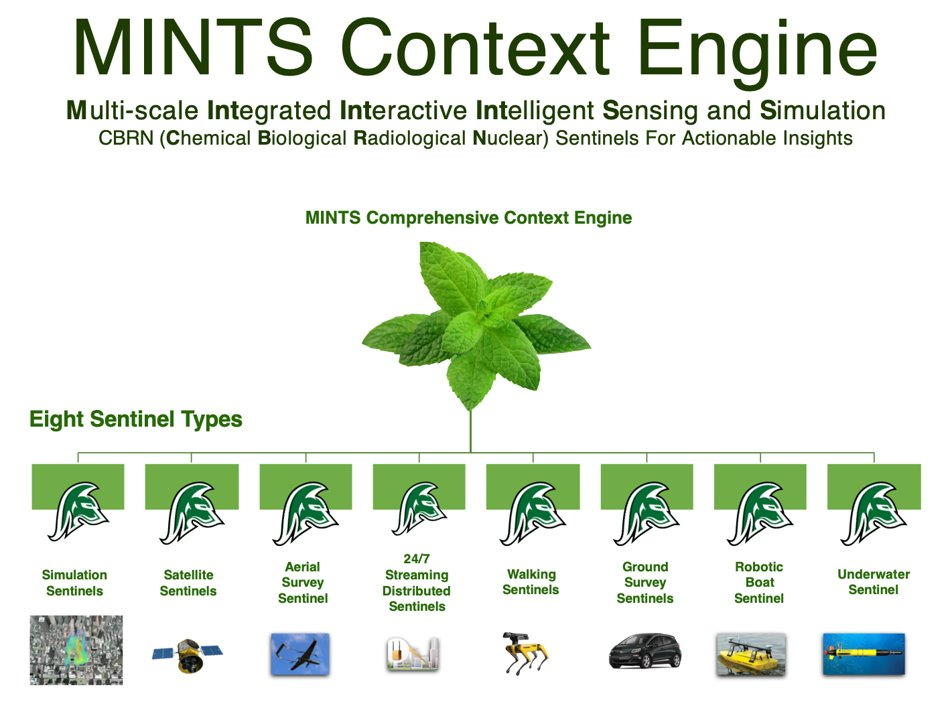
\includegraphics[width=0.8\textwidth]{introduction/MINTS-sentinels.jpg}
%   \caption{The MINTS-AI context engine is a sensing paradigm composed of flexible sensing sentinels spanning from remote sensing data products to autonomous robots and ground survey vehicles.}
%   \label{fig:mints-ai}
% \end{figure}

% Of the variety of sensing sentinels listed above, this dissertation is primarily
% concerned with three key applications. The first is a team of autonomous robotic
% vehicles which we refer to as the \textit{robotic team}. The second is a network
% of distributed streaming sentinels comprised of low-cost air quality sensors.
% The third describes a reference sensor chamber for air quality evaluation which
% we use to develop a \textit{simulation sentinel}.


% % talk here about hyperspectral imaging, in-situ water quality sensing, and
% % optical particle counters for PM as the primary sources for physical data
% \begin{itemize}
%   \item Hyperspectral Imaging
%   \item Optical Particle Counting
% \end{itemize}

% % A key challenge is that the data we measure are related nonlinearly to the
% % quantities we actually care about...


% % note about hyperspectral imaging
% In recent years, many remote sensing platforms have been deployed with
% hyperspectral imaging payloads such as the Italian PRISMA mission launched in
% 2019, the German EnMAP launched in 2022, and recently NASA's PACE satellite
% launched in 2024 \cite{PRISMA-orig, EnMAP-orig, PACE-orig}. Many future missions
% also plan to incorporate hyperspectral imaging capabilities such as the European
% Space Agency's CHIME which will include over $200$ bands spanning visible,
% near-infrared (NIR), and short-wave infrared (SWIR) wavelengths
% \cite{CHIME-orig}. The continued development of hyperspectral imaging technology
% has also led to a considerable reduction in size that enables its inclusion in
% the payloads of small unmanned aerial vehicles (UAVs)
% \cite{adao2017hyperspectral, arroyo2019implementation}. Despite the
% proliferation of hyperspectral imaging data sources, the considerable increase
% in data volume associated with hyperspectral images (HSI) poses significant
% challenges to real-time analysis at scale.






% \section{Machine Learning}

% - The Role of Machine Learning in the Era of Big Data

% Big data in the physical sciences
% Comment on the annual data volumes produced by
% \begin{itemize}
%   \item LANDSAT
%   \item Sentinel
%   \item CERN
%   \item James Webb
%   \item SDO AIA
%   \item Medical Imaging (MRI, CT scans, etc...)
% \end{itemize}

% What is machine learning

% Use of machine learning in the physical sciences

% \begin{itemize}
%   \item Remote sensing (inter-instrument calibration, classification, object identification, change monitoring via the NDVI and similar indices, etc.)
%   \item Protein Folding
%   \item Drug discovery
%   \item Surrogate modeling (i.e. for PDE solvers - now very popular at NVIDIA)
% \end{itemize}


% \subsection{Supervised and Unsupervised ML}


% \subsection{Physics-based Machine Learning}



